% !TEX root = ../thesis-example.tex
%
\chapter{Discriminator guidance}\label{sec:dg}

How to improve the generation process of a diffusion model without re-training it ? In this chapter, we will present discriminator guidance, a concept introduced by \citep{kim2023refininggenerativeprocessdiscriminator} and improved in the context of this master's thesis. Overall, this method consists in using information from a trained discriminator during the sampling process, to guide the denoising path towards the target distribution. This can be seen as a generalization of classifier guidance \citep{dhariwal2021diffusionmodelsbeatgans} to the case of the absence of class information, and can also linked to discriminator rejection \citep{azadi2019discriminatorrejectionsampling} if applied to diffusion models.
We will first start by presenting the framework proposed by \citep{kim2023refininggenerativeprocessdiscriminator} in section \ref{sec:dg:sec1}, The formulation of this framework is theoretically grounded, but the presented training scheme of the discriminator is not justified. We show in section \ref{sec:dg:sec2} that it is sub-optimal, and can worsen the sampling process in the over-fitting regime. Thus, in section \ref{sec:dg:sec3}, we propose a novel training objective that is optimal and demonstrate our results for standard generation benchmarks.
\\
In the following, we recall the notation used in our work :
\begin{itemize}
    \item $P_{t},p_{t}$ denotes the diffused \textit{target} distribution and its corresponding density at time $t$
    \item $s_{\theta}(x,t)$ denotes a \textbf{trained} score based model with fixed parameter set $\theta$
    \item $\Tilde{P}_{t},\Tilde{p}_{t}$ denotes the diffused \textit{estimated} distribution and its corresponding density at time $t$ obtained by solving \textit{exactly} the backward SDE (\ref{eq:backward_diffusion}). We assume that $s_{\theta}(x,t) = \nabla_{x}\log\Tilde{p}_{t}(x)$
    \item The trainable discriminator $d_{\phi}$ is parameterized by a set of parameters $\phi$
    \item We denote by $\pi(x)$ the density of the prior distribution used in the sampling process.
    \item The \textit{refined} distribution induced by using both the score network $s_{\theta}$ and a discriminator $d_{\phi}$ is denoted by $\Hat{P}_{t}$ and its corresponding density by $\Hat{p}_{t}$
\end{itemize}

\section{Discriminator guidance}\label{sec:dg:sec1}
\subsection{Derivation}
Discriminator guidance stems from the simple concept of estimating the training error $\nabla \log p_{t}(x) - s_{\theta}(x,t)$.
In the following, we provide a definition that would introduce a key assumption in the derivation of discriminator guidance.
\begin{definition}
    The evidence lower bound $\mathcal{L}_{\theta}$ of a score model $s_{\theta}$ is given by :
    \begin{equation}
            \mathcal{L}(s_{\theta}) = \frac{1}{2}\int_{0}^{T} \lambda(t) \mathbb{E}_{P}\left[||\nabla \log p_{t}(x) - s_{\theta}(x,t) ||^{2}  \right]dt
    \end{equation}
\end{definition}


In the following, we make the following assumption : 
\begin{assumption}\label{ass:elbo}
    The distribution  $\Tilde{P}_{t}$ induced by the backward process with score estimator $s_{\theta}$ has a log likelihood equal to the evidence lower bound of $s_{\theta}$
\end{assumption}
Define $S_{\mathrm{sol}}$ to be a family of time-conditioned score network $s_{\theta}$ that satisfies the
following: there exists densities $p_{\theta,0}$ and $p_{\theta,t}$ such that$ s_{\theta}(x, t) = \nabla log p_{\theta,t}(x)$ almost everywhere, where $p_{\theta,t}$ is the marginal density at time t of $dx = f(x, t) dt + g(t) dw$, starting from $x_{0} \sim p_{\theta,0}$
\begin{theorem}\label{thm:conservativity_score}\citep{kim2023refininggenerativeprocessdiscriminator}
    Suppose that the score network $s_{\theta}$ satisfies assumption \ref{ass:elbo}. Then $s_{\theta} \in S_{\mathrm{sol}}$. We thus denote by $\Tilde{P}_{t}$ the distribution with density $\Tilde{p}_{t}(x)$ such that $s_{\theta}(x,t) = \nabla \log \Tilde{p}_{t}(x)$
\end{theorem}



\begin{theorem}\label{theorem:dg_sde}\citep{kim2023refininggenerativeprocessdiscriminator}
Suppose that :
\begin{itemize}
    \item Assumption \ref{ass:elbo} is satisfied by the estimated score network $s_{\theta}$.
    \item  $s_{\theta}(x,T) = \nabla \log \pi(x)$.
\end{itemize}
Then, by noting $c_{\theta}(x,t) = \nabla \log p_{t}(x) - s_{\theta}(x,t) = \nabla \log \frac{p_{t}(x)}{s_{\theta}(x,t)}$, the backward SDE defined by : 
\begin{equation}\label{eq:refined_backward_SDE}
    dx = f(x,t) - \frac{1}{2}g(t)^{2}(s_{\theta}(x,t) + c_{\theta}(x,t))dt
\end{equation}
coincides with the backward SDE of the diffusion process induced by the target distribution (Equation \ref{eq:backward_diffusion}).  
\end{theorem}
The proofs for theorems \ref{thm:conservativity_score},\ref{theorem:dg_sde} are relegated to Appendix \ref{sec:appendix}.\\
Thus, if one estimates exactly the density ratio $r_{\mathrm{opt}}(x,t) = \frac{p_{t}(x)}{\Tilde{p}_{t}(x)}$, then the \textit{refined} score $s_{\theta,\mathrm{opt}}(x,t) = s_{\theta}(x,t) + \nabla \log r_{\mathrm{opt}}(x,t)$ allows for sampling from the target distribution by solving the backward SDE. \citep{kim2023refininggenerativeprocessdiscriminator} train a discriminator $d_{\phi}(x,t)$ to estimate $r_{\mathrm{opt}}(x,t)$ then computes $\nabla \log d_{\phi}$ as an estimator for $c_{\theta}$. This raises the following question : \textbf{Does a generic estimation of the density ratio make the generative process better ?}
\subsection{f-divergence between the target and refined distribution}
The following theorem follows from the conservativity of $s_{\theta}$ (Assumption \ref{ass:conservativity_refined}) : 
\begin{theorem}\label{ass:conservativity_refined}
    Suppose that the assumptions of theorem \ref{theorem:dg_sde} are satisfied. The backward SDE using as a score estimator $s_{\theta,\phi}(x,t) = s_{\theta}(x,t) + \nabla \log d_{\phi}(x,t)$ induces a distribution $\Hat{P}_{t}$ with density $\Hat{p}_{t}(x)$
\end{theorem}
\citep{kim2022maximumlikelihoodtrainingimplicit} provide an interesting result that upper bounds the Kullback-Leibler divergence between the target and refined distributions.
\begin{theorem}\label{theorem:kl_refined}\citep{kim2023refininggenerativeprocessdiscriminator}
    If the assumptions of theorem \ref{theorem:dg_sde} hold, then given the target distribution $P_{t}$, the score distribution $\Tilde{P}_{t}$ and the refined distribution $\Hat{P}_t$ we have : 
    \begin{align*}
        D_{KL}(p_{0} \| \Tilde{p}_{0}) &= D_{KL}(p_{T} \| \pi) + E_{\theta}, \\
        D_{KL}(p_{0} \| \Hat{p}_{0}) &\leq D_{KL}(p_{T} \| \pi) + E_{\phi}
    \end{align*}
    \textit{where $E_{\theta}$ is the score error}
    \[
    E_{\theta} = \frac{1}{2} \int_0^T g^2(t) \mathbb{E}_{p_{t}} \left[ \|\nabla \log p_{t}(x) - s_{\theta}(x,t)\|^2 \right] dt,
    \]
    
    \textit{and $E_{\phi}$ is the discriminator-adjusted score error}
    
    \[
    E_{\phi} = \frac{1}{2} \int_0^T g^2(t) \mathbb{E}_{p_{t}} \left[ \|\nabla \log r_{\mathrm{opt}} - \nabla \log d_{\phi}\|^2 \right] dt.
    \]
    Leading to the following inequality : 
    \begin{equation}\label{eq:gain_inequality}
        D_{KL}(p_{0},\Hat{p}_{0}) \leq D_{KL}(p_{0},\Tilde{p}_{0}) + (E_{\theta} - E_{\phi})
    \end{equation}
\end{theorem}
\citep{kim2023refininggenerativeprocessdiscriminator} provides no theoretical analysis on the positivity of the difference $ (E_{\theta} - E_{\phi})$, but argue that in practice it is initialized near 0 and gradually increases throughout training.
Table \ref{tab:dg_gain} shows the value of the difference with different initializations of the discriminator. Notably, a completely blind discriminator $d_{\phi}(x,t) = \frac{1}{2}$ has $E_{\phi} = E_{\theta}$, and an optimal discriminator has zero error. 
 \begin{table}[ht]
\centering
\caption{Discriminator-adjusted score error $E_{\infty, \phi}$ and corresponding refinement value \citep{kim2023refininggenerativeprocessdiscriminator}.}
\label{tab:dg_gain}
\begin{tabular}{@{}lcc@{}}
\toprule
Discriminator        & $E_{\theta,\phi}$ & $ E_{\theta} - E_{\theta,\phi}$   \\ \midrule
Blind $d_{\phi} (t = 0.5)$ & $E_{\theta}$      & 0             \\
Optimal $d_{\phi}$  & 0                  & $E_{\theta}$ (Maximum) \\
Untrained $d_{\phi} (\approx 0.5)$ & $\approx E_{\theta}$ & $\approx 0$  \\
Trained $d_{\phi}$  & $\ll E_{\theta}$   & $\gg E_{\theta}$ \\ \bottomrule
\end{tabular}
\end{table}
There was however no analysis in the worst case scenario, where a discriminator is \textit{badly} trained. In section \ref{sec:dg:sec2}, we present situations that are possible in practice that could make the generation process worse.




\subsection{Training the discriminator}
In order to train the discriminator, \citep{kim2023refininggenerativeprocessdiscriminator} propose the same training paradigm as in GAN training. Specifically, a discriminator is trained to minimize the binary cross-entropy loss, as suggested in the seminal GAN paper by \citep{goodfellow2014generativeadversarialnetworks} : 
\begin{equation}\label{eq:bce}
    \mathcal{J}_{CE}(\phi) = \int_{0}^{T} \lambda(t) \mathbb{E}_{P_{t}}\left[-\log d_{\phi}(x,t) \right] + \mathbb{E}_{\Tilde{P}_{t}}\left[ -\log(1 - d_{\phi}(x,t))  \right]dt
\end{equation}
and the estimated density ratio is given by $r_{\phi}(x,t) = \frac{d_{\phi}(x,t)}{1 - d_{\phi}(x,t)}$. The corresponding correction term is thus given by $c_{\phi}(x,t) = \nabla \log r_{\phi}(x,t)$. 
Training is done by generating samples from the estimated score network to estimate the second expectation in equation \ref{eq:bce}, and samples from the dataset are used to estimate the first expectation in equation \ref{eq:bce}. The main advantage this loss is providing a relatively fast training time for the discriminator.
However, no theoretical analysis is provided regarding its ability to approximate $c_{\phi}(x,t)$, that is $\nabla \log r_{\mathrm{opt}}(x,t)$. Minimizing the cross entropy loss provides indeed a good estimate for the density ratio, but not necessarily for the gradient of the log density ratio.
\\
We thus raise the following question, that we answer in section \ref*{sec:dg:sec2} : \textbf{Even if the cross-entropy is minimized, is the discriminator guidance refining the diffusion model?}

\section{Sub-optimality of cross entropy minimization}\label{sec:dg:sec2}
In this section, we first show in theorem \ref{theorem:exploding_kl} that an arbitrarily low cross-entropy loss can lead to an arbitrarily high KL-divergence between the target and refined distribution. We then show in \ref*{theorem:expectation_exploding} that over-fitting the discriminator to minimize the cross-entropy leads to a high KL divergence between $P$ and $\Hat{P}$.



\begin{theorem}\label{theorem:exploding_kl}
    Let $\left\{\vx(t)\right\}_{t\in[0, T]}$ be a diffusion process defined by Equation~\ref{eq:forward_diff}. Assume that $\nabla \log \wtp_t= \vs_\theta$ and $\nabla \log \whp_t =\vs_\theta +\nabla \log r_\phi $ and that the induced distribution $P$, $\wtP$, and $\whP$ satisfies the assumptions detailed in Appendix~\ref{sec:appendix:assumptionssong}. Then, for every $\varepsilon>0$ and for every $\delta>0$, there exists a discriminator $\vd:\reals^d\times\reals\to\reals$ trained to minimize the cross-entropy such that:
    \begin{equation}
        \calL_{\mathrm{CE}}^{d}(\phi)\leq \varepsilon \et \KL(P\Vert \widetilde{P}) \geq \delta,
    \end{equation}
    where $\widehat{P}$ is the distribution induced by discriminator guidance with $\vd$.
\end{theorem}
\begin{hproof}The detailed proof for Theorem~\ref{theorem:exploding_kl} is provided in Appendix \ref{app:sec:proofsuboptimal}. The main idea for the proof is to show that a learned discriminator $d_{\phi}$ oscillating around the true optimal discriminator $d^*$ will show a low cross-entropy. The smaller the amplitude of the oscillation, the lower the cross-entropy. However, the faster the oscillations, the larger the Kullback-Leibler divergence will be. \end{hproof}
Although theorem \ref*{theorem:exploding_kl} shows the sub-optimality of the cross-entropy, it presents a pathologic case that one cannot find in practice. In the following theorem, we consider the situation where the discriminator overfits the training data, and show that the KL divergence between the target and refined distribution can explode.
\begin{theorem}\label{theorem:expectation_exploding}
    Let $P$ and $\widetilde{P}$ be two
distributions on $\mathbb{R}$. Assume the intersection of their support
is not empty, and assume they admit density functions $p$ and $\tilde{p}$
which are both $L$-Lipschitz. Let $x_{1}\ldots x_{N}\sim P^{N}$
and $x_{1}'\ldots x_{N}'\sim\tilde{P}^{N}$. Assume that the or cross-entropy loss $-\log\sigma\left(d_{\varphi}(x_{i})\right)$
and $-\log\left(1-\sigma\left(d_{\phi}(x'_{i})\right)\right)$
is at most $\epsilon$ on each example $x_{i}$ and $x_{i}'$. Then,
the expectation over the dataset of the mean square error exhibits
the following behavior, for some constant $c$:
\begin{equation}
    \lim_{N\rightarrow\infty}\frac{\mathbb{E}\left[E_{\phi}\right]}{N}\to c.
\end{equation}
In other words, the difference $E_{\theta} - E_{\phi}$  decreases linearly with the number of samples. This shows that the upper bound on the KL divergence between the target and refined distribution goes to $-\infty$ in an over-fitting regime.
\end{theorem}
\begin{hproof}The Theorem is proved in Appendix~\ref{sec:app:proofoverfitting}. While we assume a one-dimensional diffusion process for the sake of simplicity, this result could be applied to higher dimensional. The key argument is to show that if the discriminator is overfitting the cross-entropy, the values of $d_\phi$ on real and fake samples will be very different. However, the closer the distributions $P$ and $\whP$, the higher the probability of sampling a fake sample that is close to a real sample. Therefore, the discriminator gradient will be high between the two samples independently of the true gradient value.
\end{hproof}

Intuitively, these results are due to the fact that \citep{kim2023refininggenerativeprocessdiscriminator} provide a good estimation for the density ratio $\frac{p_{t}(x)}{\hat{p}_{t}(x)}$, but not for the gradient of the log density ratio.
This raises the following questions:
\begin{itemize}
    \item \textbf{How can we train the discriminator to provide a good estimate for the gradient of the log density ratio ?}
    \item \textbf{Instead of training a model to estimate the density ratio, can we train a model to directly estimate the gradient of the log density ratio ?}
\end{itemize}
\section{Improving the refinement process}\label{sec:dg:sec3}
In this section, we answer the first aforementioned questions by deriving an optimal loss for the refinement problem.
Similarly to \citep{vincent_connection_2011,song2021scorebasedgenerativemodelingstochastic}, we propose a denoising score matching loss to estimate $\nabla \log r_{\mathrm{opt}}(x,t)$, and prove that minimizing our proposed loss minimizes the KL divergence between the target and refined distribution. We furthermore provide a few experiments to demonstrate the effectiveness of our method on image generation benchmarks.
\subsection{Denoising score matching loss}
In order to focus on estimating the gradient of the log-density ratio, we propose to minimize the following score matching loss : 
\begin{equation}\label{eq:refinement_score_matching}
    \mathcal{J}_{SM}(\phi) = \int_{0}^{T} \lambda(t) \mathbb{E}_{P_{t}}\left[||\nabla \log p_{t}(x) - s_{\theta}(x,t) - \nabla d_{\phi}(x,t) ||^{2}  \right]dt
\end{equation} 

However, the density $p_{t}(x)$ is intractable in practice, thus we propose the following \textit{MSE} loss, similar to the proposed loss of \citep{vincent_connection_2011,song2021scorebasedgenerativemodelingstochastic} :
\begin{equation}\label{eq:refinement_mse}
    \mathcal{J}_{MSE}(\phi) = \int_{0}^{T} \lambda(t) \mathbb{E}_{{t}}\left[ \mathbb{E}_{x_{0}\sim P_{0}} \left[ \mathbb{E}_{x_{t}  \sim P_{t}_{|x_{0}}} \left[  || \log p_{t}(x_{t}|x_{0}) -  s_{\theta}(x,t) + \nabla d_{\phi}(x,t) ||^{2} \right] \right] \right] dt
\end{equation}
The following proposition states that miniming $\mathcal{J}_{MSE}$ is equivalent to minimizing $mathcal{J}_{SM}$. 
\begin{proposition}\label{theorem:optimality_mse_sm}
    Assume that $P$ and $\wtP$ satisfy the assumptions detailed in Appendix~\ref{sec:appendix:assumptionssong}.
    Then, the following holds:
    \begin{equation}
        \argmin_\phi \mathcal{J}_{\mathrm{SM}}(\phi) = \argmin_\phi \mathcal{J}_{\mathrm{MSE}}(\phi).
    \end{equation}
\end{proposition}
\begin{hproof}
The proof is provided in Appendix \ref{sec:app:proofmseloss}, and is based on the fact that the two losses are equal up to an additive constant.
\end{hproof}
\begin{figure}[t]
    \centering
    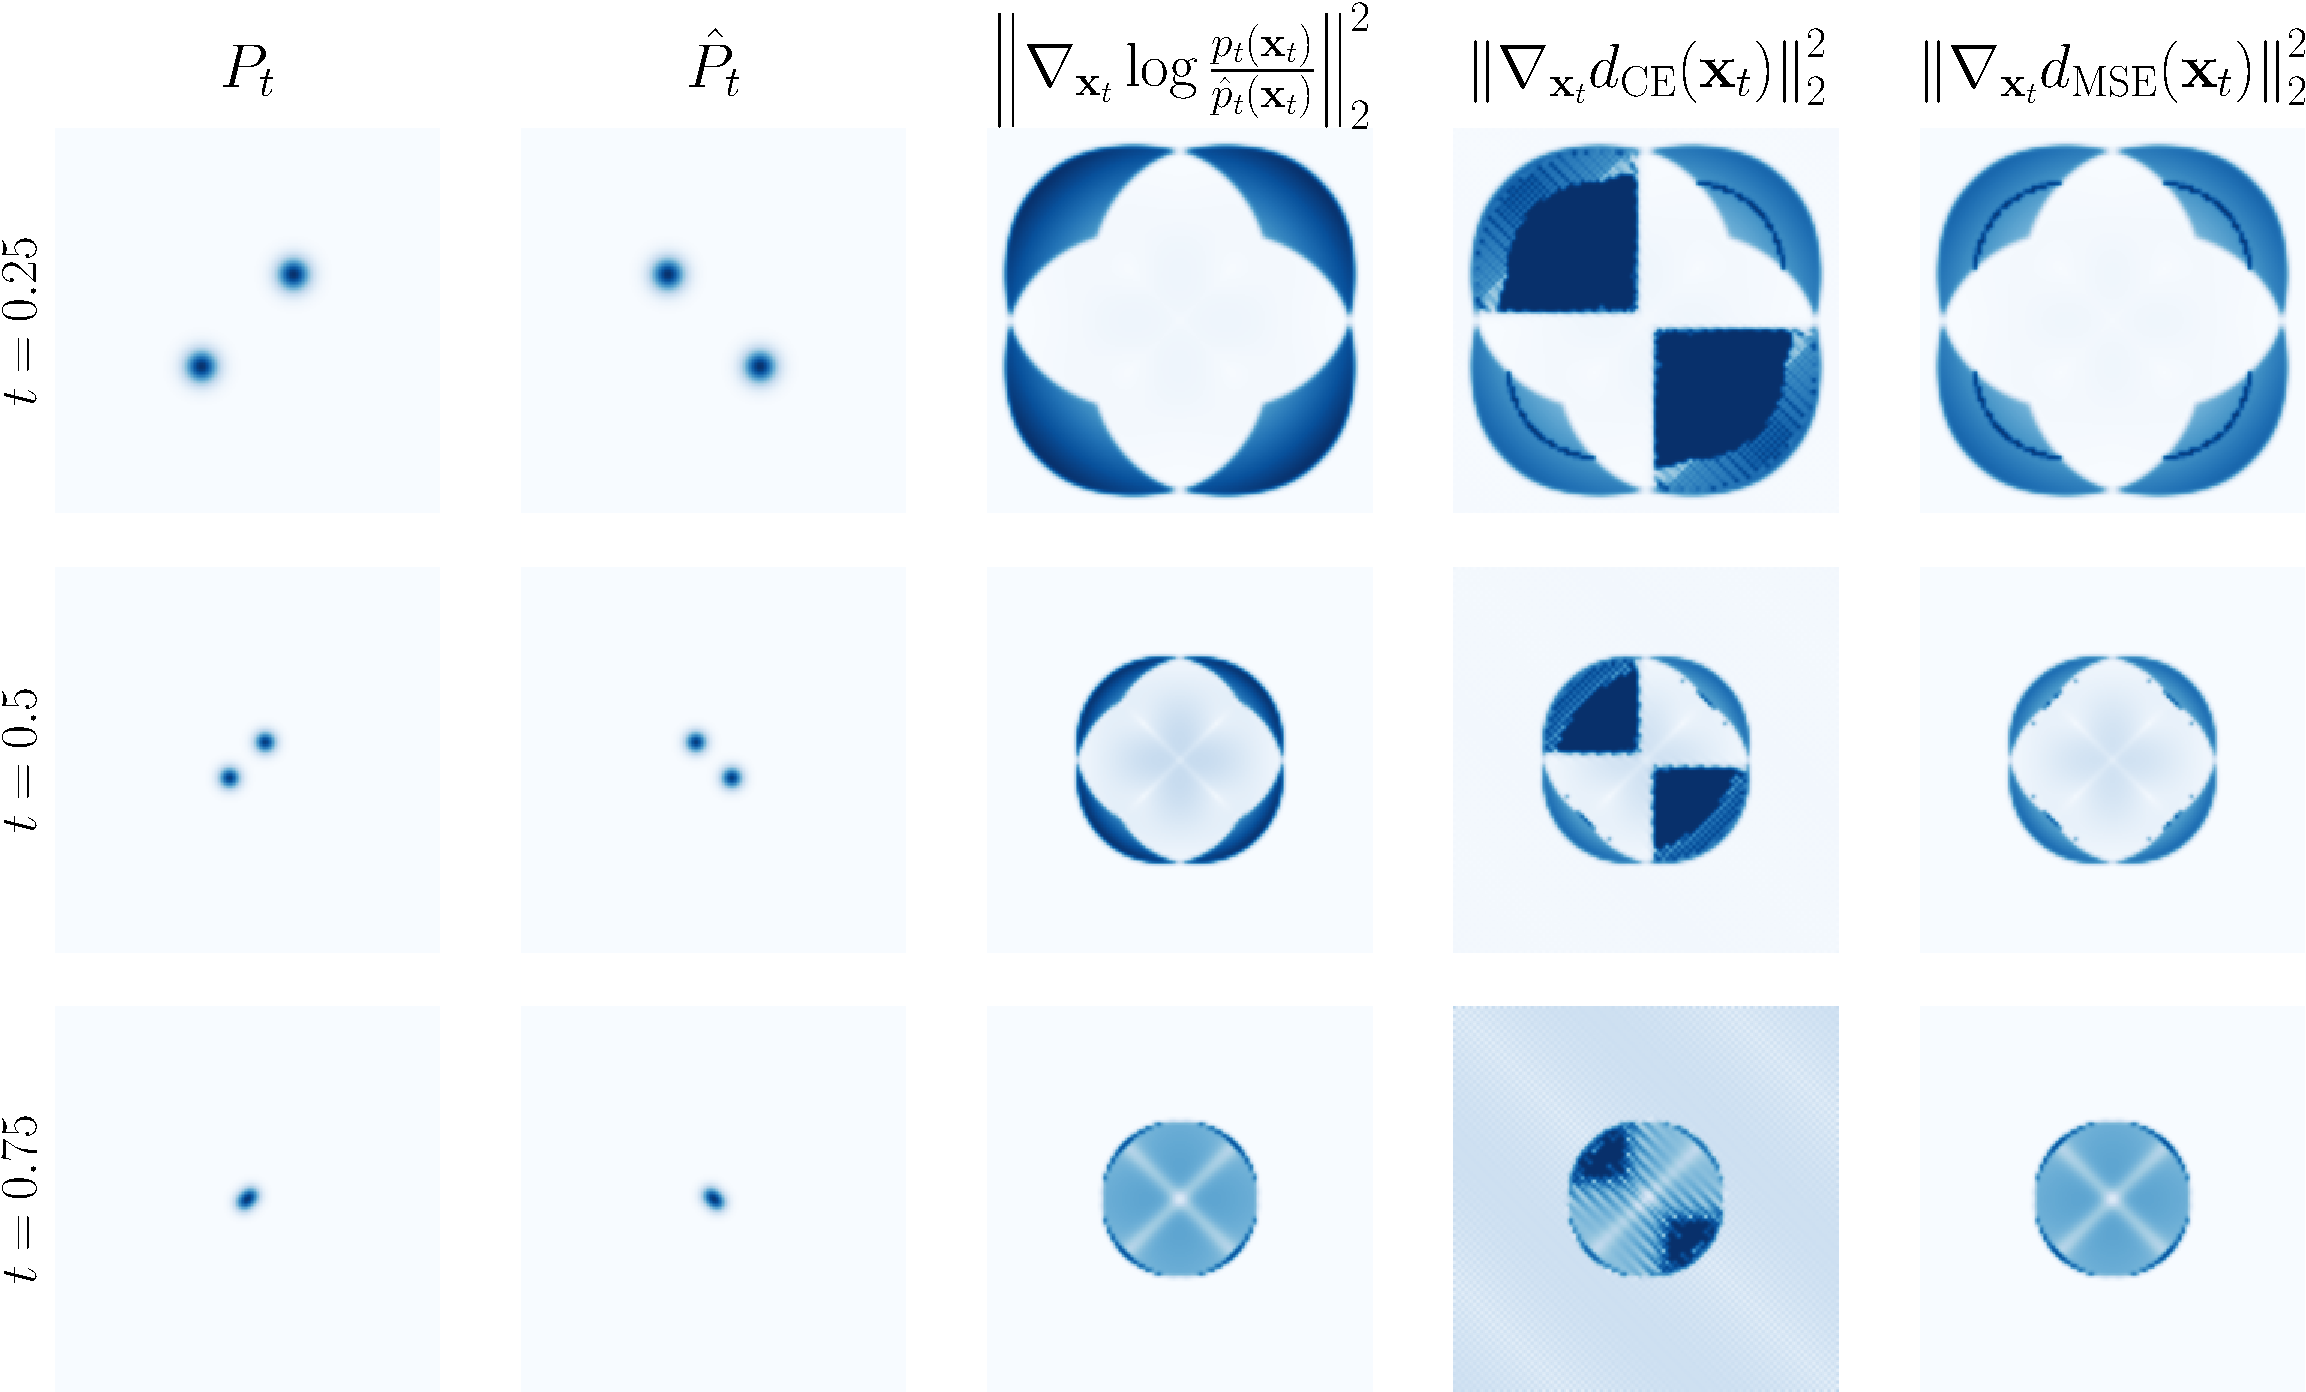
\includegraphics[width=\textwidth]{gfx/gradients_wrt_ts.pdf}
    \caption{Visualizing the estimation of $\nabla_{\vx_{t}} \log p_{t}(\vx_{t})/\nabla_{\vx_{t}} \log \hat{p}_{t}(\vx_{t})$ for the discriminator trained with low cross-entropy or low MSE loss. We plot the norm of the gradient for better readability. We can see here that the discriminator trained on minimizing $\mathcal{J}_{CE}$ provides a poor estimate of the gradient, while the one trained on $\mathcal{J}_{MSE}$ provides a sound estimate.}
    \label{fig:2d_gradient}
\end{figure}
\begin{figure}[t!]
    \centering
    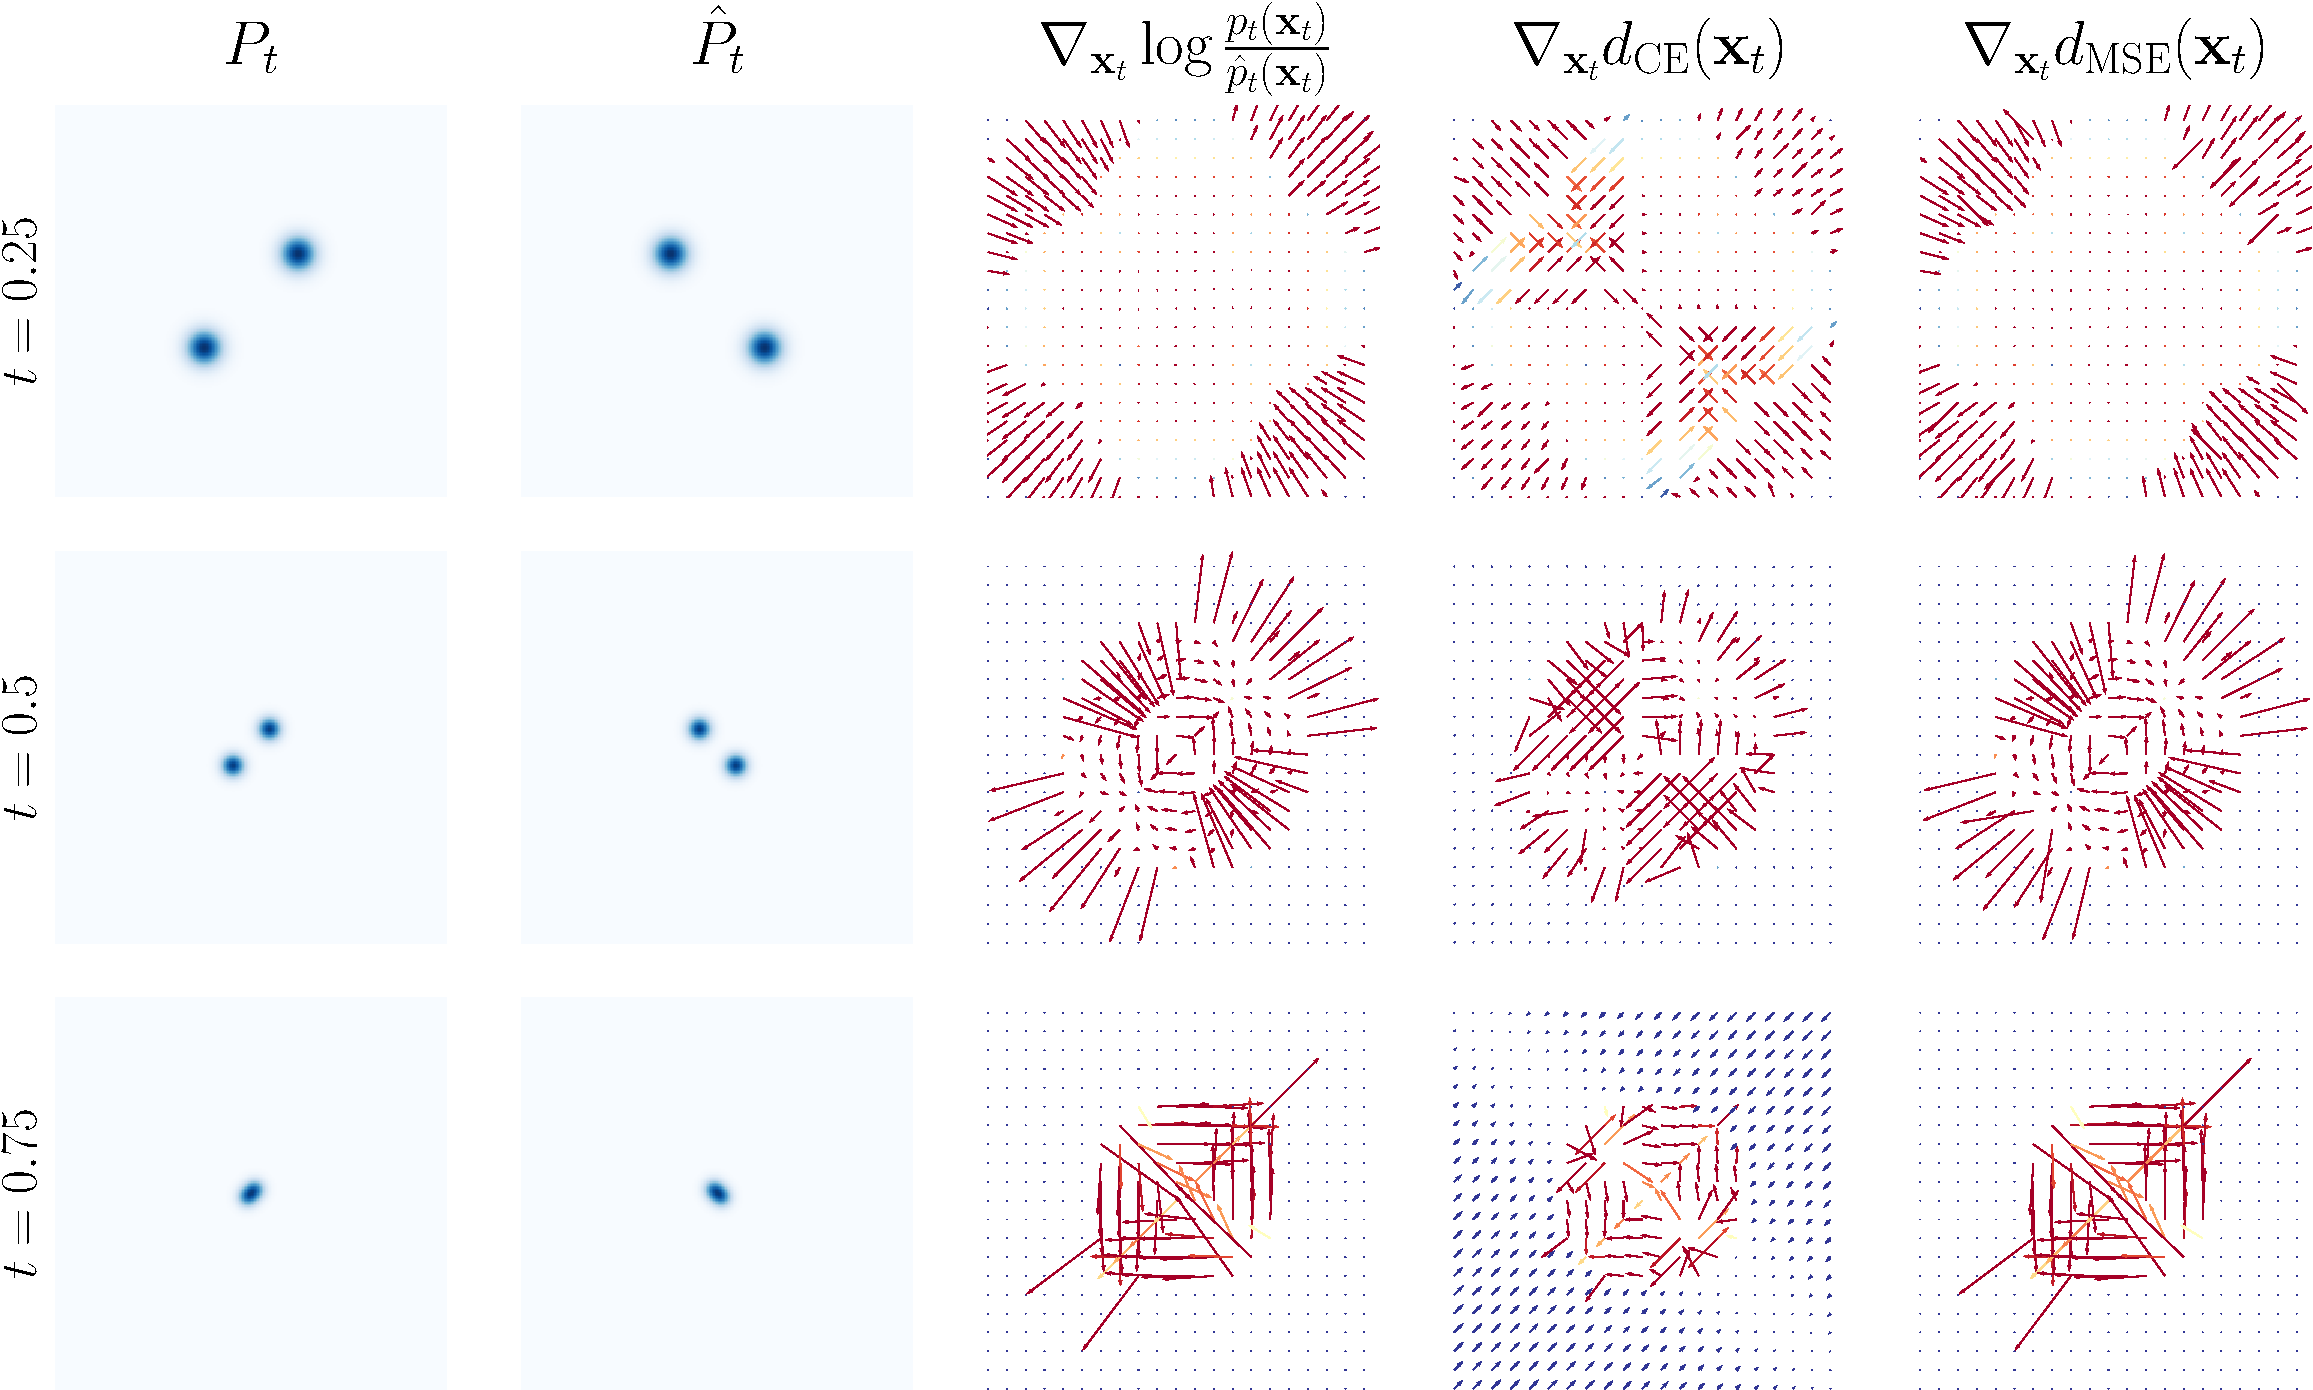
\includegraphics[width=\linewidth]{gfx/quivers_wrt_ts.pdf}
    \caption{Gradients of the estimated density ratio. $d_{\mathrm{CE}}$ represents a discriminator with low cross entropy, and $d_{\mathrm{MSE}}$ represents a discriminator with low MSE}
    \label{fig:2D-quivers}
\end{figure}
\subsection{Practical considerations}
One advantage proposed by the approach of \citep{kim2023refininggenerativeprocessdiscriminator} is the usage of generated samples from $\Hat{P}$ at each training step. 
Training a discriminator to minimize the MSE loss is more prone to overfitting, as no new samples are generated during training, as opposed to the cross-entropy loss. Furthermore, as our work focused on improving generation for already well trained model, the error $\nabla \log \frac{p_{t}(x)}{\tilde{p}_{t}(x)}$ is small. We thus propose to use leverage the generative abilities of the pretrained diffusion model $s_{\theta}$ to gain more information, by adding $\mathcal{J}_{CE}$ as a regularization term: 
\begin{equation}
    \mathcal{J}_{\mathrm{train}}(\phi) = \mathcal{J}_{\mathrm{MSE}}(\phi) + \gamma\mathcal{J}_{\mathrm{CE}}(\phi)
\end{equation}
where $\gamma$ is a hyperparameter controlling the regularization strength.
\section{Experiments}
\subsection{Toy example}

\textbf{Setting:}We consider two distinct mixtures of Gaussians in $\reals^{2}$, that represent respectively $P$ and $\tilde{P}$. We compute for a subset of timesteps $t \in [0,1]$ the closed form of the scores $\nabla_{\vx_{t}} \log p_{t}(\vx_{t})$ and $\nabla_{\vx_{t}} \log p_{t}(\vx_{t})$, and we use them for performing a discretized backward diffusion process. In order to concentrate on the effect of discriminator guidance, we first sample points from $P$, perform a forward diffusion process using subVP-SDE \citep{song2021scorebasedgenerativemodelingstochastic}, and start from this set of points as a prior distribution. 
\begin{figure}[b!]
    \centering
    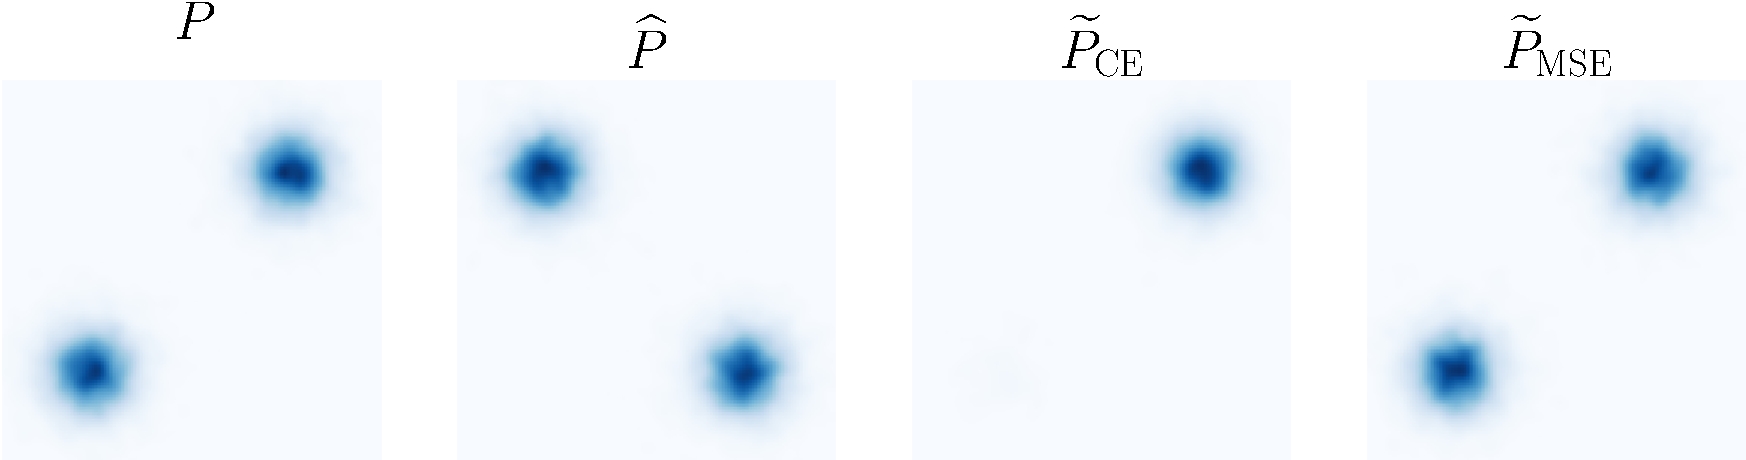
\includegraphics[width=\textwidth]{gfx/3_scenarios_omega_1e4.pdf}
    \caption{Comparison of the sampling process by using a discriminator to minimize the cross-entropy loss defining a distribution $\Tilde{P}_{\mathrm{CE}}$ and a discriminator to minimize the MSE loss $\mathcal{J}_{\mathrm{SM}}(\phi)$ defining a distribution $\Tilde{P}_{\mathrm{MSE}}$. We can see that the cross entropy loss misses one mode of the target distribution}
    \label{fig:2Dplots}
\end{figure}

\textbf{Evaluation of the optimization procedure :}
We also compute two estimations of the discriminator. The first estimate $d_{\mathrm{CE}}$ is based solely on minimizing $\mathcal{J}_{\mathrm{CE}}$ and the second $d_{\mathrm{MSE}}$ ensures a small $\mathcal{J}_{\mathrm{MSE}}$. We plot in Figure \ref{fig:2d_gradient} the gradient estimates across the denoising process and show that the discriminator estimated by minimizing the cross-entropy has a bad gradient estimate. Figure \ref{fig:2Dplots} shows that the failure to accurately estimate the gradient is detrimental to the denoising process. We also provide in Appendix \ref{fig:2D-quivers} the gradient plots of the different estimates.
\begin{figure}[b!]
    \centering
    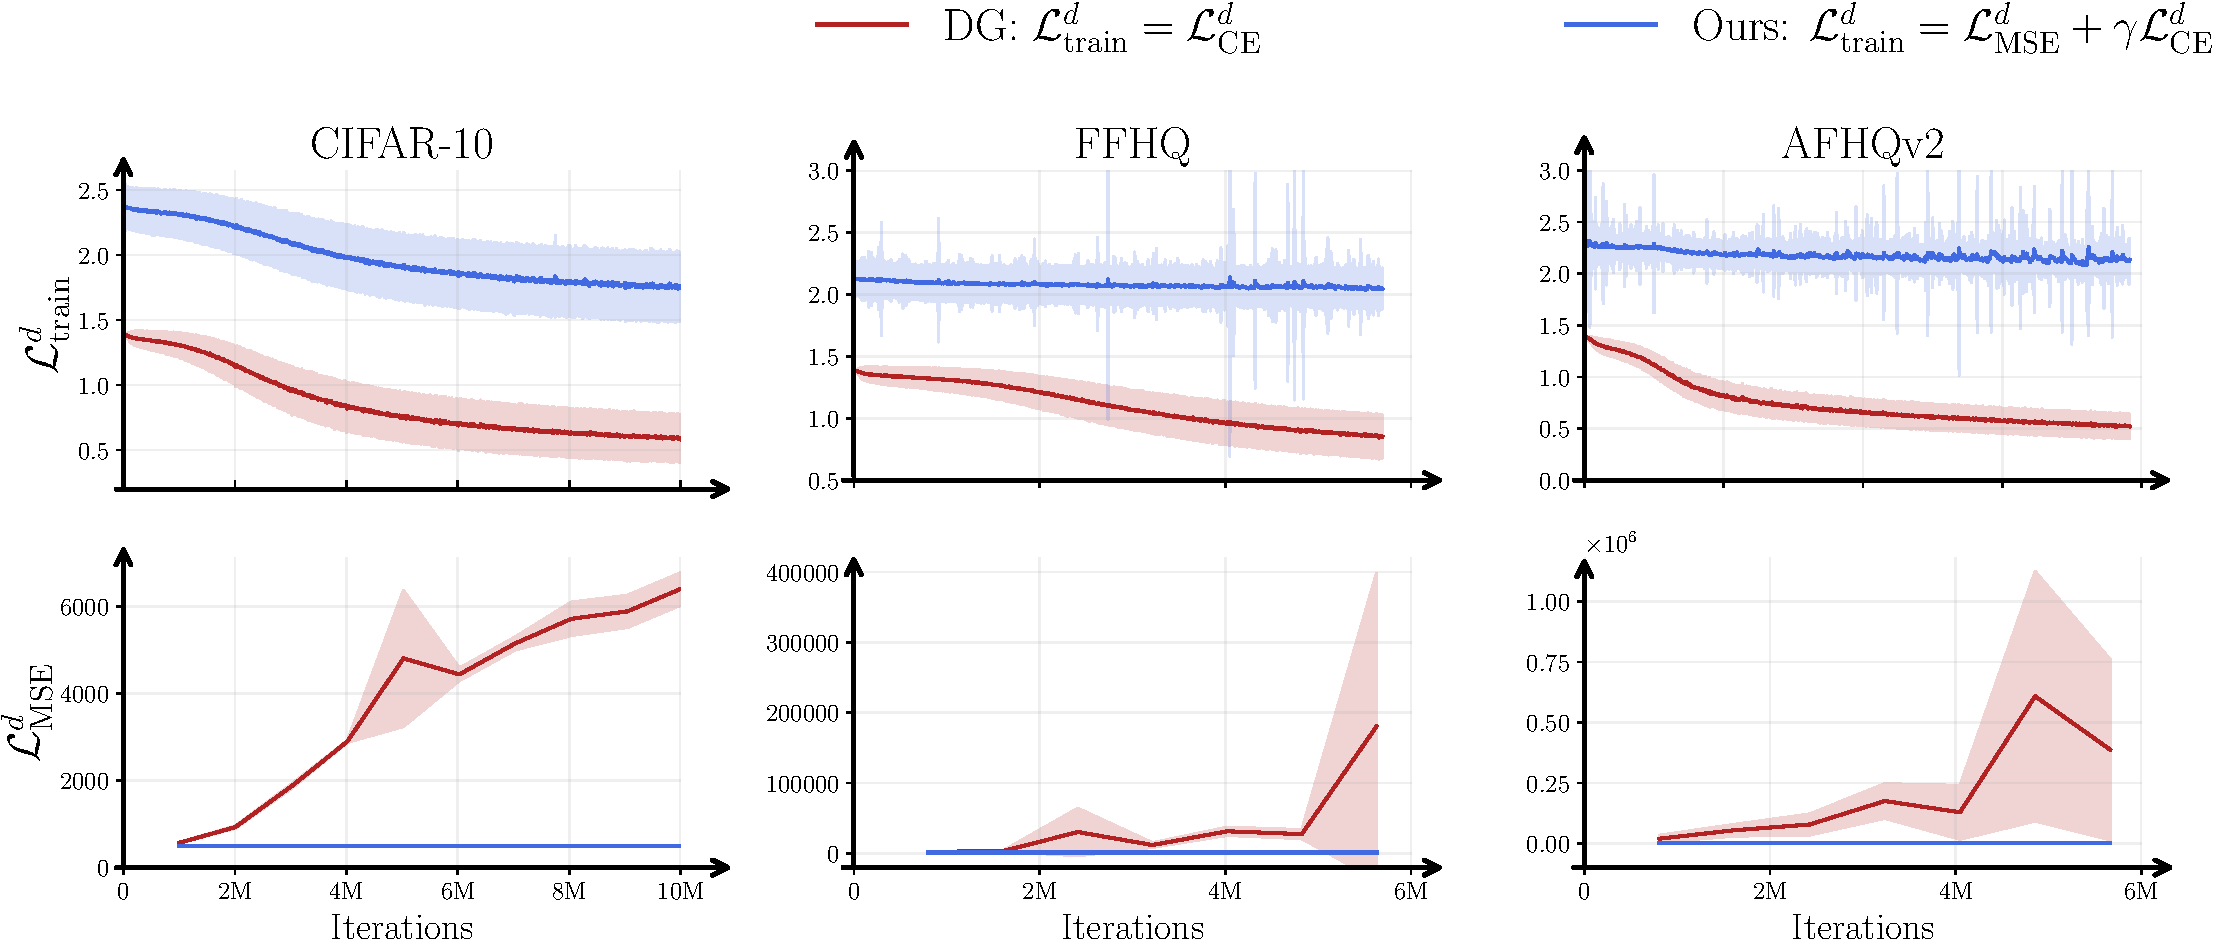
\includegraphics[width=\textwidth]{gfx/losses_DGvsOurs.pdf}
    \caption{Comparison of the proposed method with the method of \citet{kim2023refininggenerativeprocessdiscriminator} on the EDM model \citep{karras} on CIFAR-10, FFHQ and AFHQ-v2 datasets. For the method proposed by \citet{kim2023refininggenerativeprocessdiscriminator}, denoted as DG, the MSE loss $\mathcal{J}_{\mathrm{MSE}}$ increasing during training. The proposed method, denoted as Ours, shows a stable behavior. The error bars represent the standard deviation over 3 runs.}
    \label{fig:losses}
\end{figure}
\subsection{Image generation}
We implement our approach using the pre-trained EDM model \citep{karras}. We will compare our approach with the pre-trained models (EDM) and the pre-trained models with discriminator guidance (EDM+DG). For a fair comparison to \cite{kim2023refininggenerativeprocessdiscriminator}, we build the same architecture for the discriminator $d_\phi$ using pre-trained embedding of the ADM classifier models used in the work of \citet{dhariwal2021diffusionmodelsbeatgans}. However, our method requires using the same framework as EDM, therefore we reimplemented DG for various datasets and resolutions. We use the same hyperparameters as \citet{kim2023refininggenerativeprocessdiscriminator} for the discriminator guidance method, and we apply both methods on the CIFAR-10, FFHQ and AFHQ-v2 datasets on, respectively, 8x GPU-V100, 8x GPU-A100 and 8x GPU-A100. First, we illustrate the behavior of the training loss ($\mathcal{J}_{\mathrm{CE}}$ for DG and $\mathcal{J}_{\mathrm{train}}$ for Ours) and the reconstruction loss during training in Figure~\ref{fig:losses}. We can see that our approach enables us to mitigate the increase of the MSE loss, while the DG method shows a clear increase of the loss. However, we observe a decrease in the training loss that demonstrates that the density ratio is learned.

We report the FID\footnote{Note that we can observe some discrepancies between the results in \cite{kim2023refininggenerativeprocessdiscriminator} due to the reimplementation of the framework to closely match the generative process of EDM} \citep{heusel_gans_2017}, Precision and Recall \citep{kynkaanniemi_improved_2019} scores in Table~\ref{tab:results}. Metrics are computed using the Guided Diffusion library \citep{dhariwal2021diffusionmodelsbeatgans} using 50k samples for CIFAR-10 and FFHQ, and 15k samples for AFHQ-v2. We use $k=5$ to compute the Precision and the Recall. We can see that our method systematically outperforms the DG method on all datasets even if the difference with the EDM model is small.    

\begin{table}[t]
\centering
\caption{Comparison of the proposed method with the method of \citet{kim2023refininggenerativeprocessdiscriminator} on CIFAR-10, FFHQ and AFHQv2. We give metrics averaged on 3 trainings procedure with one standard deviation.} \label{tab:results} 
\begin{tabular*}{\textwidth}{lcl@{\extracolsep{\fill}}ccc}
\toprule
Dataset & Resolution & Method & FID & P & R \\
\midrule
\multirow{3}{*}{CIFAR-10} &\multirow{3}{*}{{$32\times32$}}&  EDM & $2.03$ & $99.12$ & $76.84$\\
 && EDM + DG & $3.03 \pm 0.05 $ & $99.06 \pm 0.10 $ & $72.56 \pm 0.14 $ \\
 && EDM + Ours & $2.00 \pm 0.01 $ & $99.18 \pm 0.04 $ & $76.70 \pm 0.12 $ \\
\midrule
\multirow{3}{*}{AFHQv2} &\multirow{3}{*}{{$64\times64$}}&  EDM & $2.62$ & $99.92$ & $84.66$\\
 && EDM + DG & $2.66 \pm 0.02 $ & $99.92 \pm 0.00 $ & $83.70 \pm 0.22 $ \\
 && EDM + Ours & $2.61 \pm 0.00 $ & $99.92 \pm 0.00 $ & $84.62 \pm 0.01 $ \\
\midrule
\multirow{3}{*}{FFHQ} &\multirow{3}{*}{{$64\times64$}}&  EDM & $2.54$ & $99.75$ & $78.85$\\
 && EDM + DG & $2.63 \pm 0.03 $ & $99.74 \pm 0.02 $ & $77.55 \pm 0.06 $ \\
 && EDM + Ours & $2.54 \pm 0.00 $ & $99.75 \pm 0.00 $ & $78.87 \pm 0.02 $\\
\bottomrule
\end{tabular*}
\end{table}
\subsection{Comments on the results}
Training a discriminator to refine the EDM model \citep{karras} slightly improved the generation metrics, but the difference is not significant. We hypothesize that this is due to the fact that the EDM model is already well trained, and the discriminator guidance method is not able to provide a good estimate of the gradient of the log-density ratio. A more notable contribution would be to try this method on less trained models, and evaluate the improvement in FID, precision and recall. 
Thus, as future directions of this part, we propose the following : 
\begin{itemize}
    \item Our work also lacks the diversification of architectures, and should have been tried with other pre-trained models, for tasks different than image generation.
    \item Fine-tune the hyperparameter $\gamma$, or investigate other regularization terms to improve the training process.
    \item Restrict discriminator guidance to timesteps $t$ where the score estimation is poor.
    \item Investigate the effect of discriminator guidance on less trained models.
\end{itemize}

\section{Conclusion}\label{sec:dg:conclusion}
In this chapter, we presented a method for refining pre-trained diffusion models using a smaller discriminator network. After introducing the method proposed by \citep{kim2023refininggenerativeprocessdiscriminator}, we provided theoretical results that lead to modifying the training objective of the discriminator, and prove that our proposed objective is optimal.
We then provided experimental results to evaluate the validity of our approach, and showed that it was not effective for the EDM model. We provided future directions to improve the method. 
Discriminator guidance attempts to correct the \textit{approximation} errors related to the score estimation while training. Now, the following chapter answers the following question : \textbf{Can the sampling erros, related to the discretization of the backward process, be corrected by a boosting method ?}

